\section{Design}
As a dialogue agent, a chatbot needs to be designed with conversation with a human user in mind, with each turn in the exchange serving a function of supplying or retrieving information from the system. \\
To determine what kind of interactions the users and the chatbot should have, we started our design phase using the Botmock tool to draft some conversation graphs.
One consideration when determining the tonality of our conversation sketches was determining what personality the chatbot should exhibit. Since chatbots users have shown to appreciate the fun aspect of designed chatbot personalities \cite{10.1007/978-3-319-67744-6_28}, we tried to imbue our conversations with some colloquial aspects, like using slang, calling the user names, and using emojis. Additionally, we added some level or randomisation to the stock responses we would give, to make sure the chatbot didn't feel repetitive, especially for frequent expressions. \\

\begin{figure}[h!]
  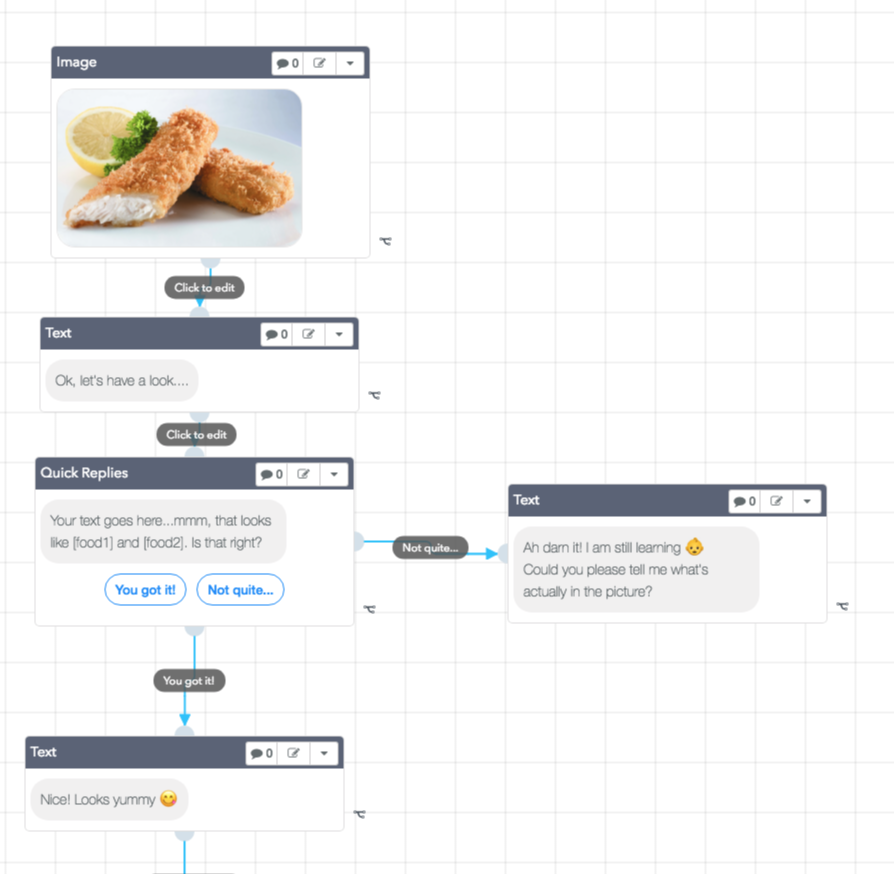
\includegraphics[width=\linewidth,keepaspectratio]{Botmock.png}
  \caption{An example conversation flow drafted in Botmock}
\end{figure}

To establish a level of familiarity, rather than fetching a user's name from the client's account information, we initiate our first conversation by asking for it. The rest of the introductory messages just describe the chatbot's functionalities.
Besides asking for help, users have three main available actions they can take: tell the chatbot what they are eating, send a picture of food, and ask the chatbot to recap what they had on a specific date. If the user doesn't specify a quantity or measurement to their meal, the chatbot will ask for details. To avoid bogging down the user with measuring their portions, and since we mostly want them to think about their diet in general terms, we encourage to use relative rather than absolute quantities (more, less or same as usual). We hope that using these measurements we will be able to maintain longer term user engagement, without sacrificing understanding of how much food is being consumed. Once we have this information, we send it through the Nutritionix API, to find out the nutritional content of that meal. \\
Sending a picture to the chatbot triggers a call to the \textit{clarifai} vision API, to understand what the contents of the image is, using their food model. \textit{clarifai} returns a list of guesses for a picture, and their confidence value. If only one guess has confidence above the arbitrary threshold of 97\%, we save the food in the picture in our database; in any other case, we present the user with a list of the top three guesses as interactive buttons, so we can store the correct value in the database. \\
\subsection{Nutritional analysis}
Once the user starts logging details about their food consumption, we will need to start analysing what they are eating to give them advice. Lacking comprehensive nutritional knowledge, the best we can do is crafting some elementary heuristics. \\
The food retrieval intent queries the chatbot's database for all foods stored on a certain date. To aid user's reflection, we provide some basic data analysis, specifically on the food's quantity: if there are more than 10 foods logged, with at least one having been consumed in large quantities and either less than two thirds consumed in small quantities or more than two thirds consumed in large quantities, we warn the user they might be overeating. Conversely, if they have logged less than 3 items of food, or if more than $2/3$ of their meals come in a small quantity, we warn the user about undereating. If they are asking about the current date, they might just not have had time to log all their food; in that case, we only send a warning if the current time is past 10 PM.\\
One example of food category that is often praised by nutritionists for its high nutritional value \cite{} is leafy green vegetables. To demonstrate the capabilities of chatbots as nutritional advisers, we handcrafted a list of leafy greens, which we check every meal for. If we don't observe the user eating any of these foods in 2 days, we prod the user with a reminder. Prodding in a chatbot context requires finding a very delicate balance: it can be too infrequent, making it less useful for users who actually want to be reminded; but if too frequent, it  might soon become annoying. For example, the Forksy nutritional chatbot \cite{forksywebsite} sends a reminder to log a meal for every single one (at least 3 a day). This causes the bot to feel overbearing, and it might actually drive the user away (Forksy actually implements an interesting solution by asking how long before the next reminder, but it still gives no option to deactivate reminders completely). Our solution is staggering the no usage messages at increasing intervals, first after day one, then on day two, four, seven and fifteen, to maximise our chances of getting a forgetful user to start messaging again, without being too annoying if they choose not to. Larger amount of data analysis might be used in the future to determine when, based on current dietary habits or external inputs, the notification might be more effective in nudging the user into resuming logging or eating vegetables, and eventually provide an overall more active prompting system that takes into account correct dietary practices.

\section*{Architecture}
Our chatbot's architecture is composed of a natural language interface in Google Dialogflow, hooking up to an Express.js server running a Heroku instance, storing data on a hosted MongoDB, and retrieving other information from external APIs. The agent itself is presented through a Facebook Messenger bot, which we chose for its popularity.
\subsection*{Dialogflow concepts}
Today there are several Natural Language Understanding platform specifically designed to create chatbots. Our choice fell on \textit{Google Dialogflow} (at the time \textit{API.AI}), because of its ease of integrations with most popular messaging platform, ease of development and solid NLP functionality. A Dialogflow agent is set up with a library of patterns, \textit{intents}, that use example sentences or templates to parse inputs to the chatbot. Templates include parameters whose types are called \textit{entities}, some of which are already defined by Dialogflow, but new ones can also be added by the programmer. One of the standout capabilities of Dialogflow is that a parameter can be marked as required by the intent, so if the initial utterance does not contain it, the chatbot will prompt the user to specify the new parameter. To maintain the flow of conversation, an intent can be followed by another, based on what the user replies, with a context object which stores all parameters passed from the original intent down to all its followups. Each intent can trigger an immediate response, as defined on the Dialogflow console, or it can trigger an \textit{Action} to be fulfilled by the \textit{Webhook}. \textit{Actions} are functions held on the server that can access the parameters of the current intent, execute their own logic, call external APIs etc. They usually are triggered as a POST request to the webhook's address, with the request JSON object as its body, and the HTTP response determines the behaviour of the chatbot, either by replying with more text, sending media or rich text, or triggering an \textit{event}, which executes an intent just as one of the triggering sentences had been sent by the user. Small talk intents are also defined as part of Dialogflow to take care of common sentences unrelated to the chatbot's domain, and Dialogflow's machine learning engine can be interacted with through a Training console (still in Beta at the time of writing), which can be used to correct intent and parameter recognition (and indirectly, to gain insight into how the engine's model classifies new text).

Our chatbot defines the following intents:
\begin{itemize}
  \item \textit{First interaction} is the initial intent, triggered by the Facebook Messenger "Get Started" button or with the "Greetings" keyword for debugging purposes. This asks the user what their name is, and is followed up by 
  	\subitem \textit{Name save} which waits for a name to be given, and saves it to the database
        \subitem \textit{Name confirmed} replies with a welcome explanation message
\item \textit{Food log - text} is triggered when the user adds a meal to the log. It takes required parameters of food (as a list), quantities, and optional parameters of meal name and date
\item \textit{Send food pic} waits for a Facebook Messenger Media object (a picture in our case) to trigger an action which runs image recognition. If no unique match is found, 
  \subitem \textit{Send food pic - no} is triggered by the webhook whenever there is no clear candidate for classification of a picture
  \subsubitem \textit{Clarify food pic} recognises user's sending a clarification for what the food was through a Facebook Messenger button. To make sure the button's message matches this intent and not the generic food logging, a messenger\_button token is appended to the message payload
  \subitem \textit{Send food pic - yes} is launched whenever a picture is classified correctly, and just triggers the Analyse food pic intent
  \subitem \textit{Analyse food pic} takes the food content found in a picture received from the user, analyses and stores the result into a database
  \item \textit{Help} matches a request for help with a few reminders of the chatbot's functionalities
  \item \textit{Date retrieval} is used to query for past food logs, taking just a date as a parameter. For logging purposes, with removal functionality to be implemented in the future,
	  \subitem \textit{Date retrieval - false} will recognise when the user declares the food log for that day to be incorrect
  \item \textit{What's my name} is mainly a debugging intent, to check if the chatbot has managed to successfully save the name for the current user in the database
  \item \textit{Sinkhole} is used for training purposes to redirect all the intents that were misclassified
\end{itemize}
Our chatbot defines the following entities:
\begin{itemize}
  \item \textit{meal} enumerates four different meals: breakfast, lunch, dinner and snacks
  \item \textit{quantity} contains a list of all the different measurement units for food
  \item \textit{meal-quantities} combines quantities with quantifiers (a, some, integers etc.)
  \item \textit{approximate-quantifier}
  \item \textit{date-ext} extends the @sys.date object with today and tomorrow
\end{itemize}

\subsection*{Backend}
By default, the Dialogflow interface includes a small inline editor to implement some simple webhook logic. While the web interface is limiting for creating a backend of the complexity required, it's easy to export this example code to Google Cloud Functions \cite{gcfwebsite}, Google's serverless cloud function service, and their own database, storage and analytics tool, Firebase. 
The sample code consists of an Express.js \cite{expresswebsite} web server, which listens to POST requests to the \textit{/webhook} route to the server, which will be sent from Dialogflow, and provides helper functions to craft the appropriate response as a JSON object, which will trigger a reply through the chat client. The largest portion of the code is the action-handlers dictionary, which associates a different function to any of the Dialogflow intents. \\

We started developing our webhook from this starting example in GCF, but we soon realised that a core requirement of our design, the ability to call up external APIs, was not possible under the free tier of Google Cloud. Thus, it was necessary to find a replacement. Some options that were considered were Apache OpenWhisk \footnote{https://openwhisk.apache.org}, Captain Duck Duck \footnote{https://github.com/githubsaturn/captainduckduck}, Amazon Web Service Lambda or Elastic Beanstalk \footnote{https://aws.amazon/com/products}, Dokku \footnote{https://github.com/dokku/dokku}, 1backend \footnote{https://github.com/1backend/1backend}. In the end, Heroku was selected as a solution because of its many productivity advantages. Among the many alternative the popular Platform as a Service (PaaS) solutions offer, we took into consideration the mature tooling, the easy to use deployment infrastructure, which consist of simply pushing the code to a version controlled repository, the automatic inclusion of a free domain name, and simple (but barebone) scheduling functionality. Heroku offers both a free and a paid tier; for our purposes of creating a prototype, the free tier offers all required functionality; however, it would not be sufficient to power the chatbot infrastructure in a production setting, as there are limits to free users' capabilities, most notably a temporary suspension (and prolonged wake up times) after an hour of inactivity.
Having moved to a full PaaS implementation, we were able to expand our program from a single file to several modules, which was necessary to avoid a large unwieldy single file, and allows us to compartmentalize between different types of functionality.
\begin{itemize}
  \item \textit{index.js} is the main function for the Express server, it runs in a loop waiting to receive any requests, and serves a response for any predefined URLs. On a POST request to \textit{/webhook}, it will read the request body to find the action's name and parameters, and calls a function as defined in the \textit{actionHandlers} dictionary. Most intents match one-to-one to an inline function in this object, although some are defined in an external module
  \item \textit{messenger.js} contains output functions to send a reply to the user, either going through the Dialogflow API, or directly through the user's Facebook Messenger account (necessary for sending a message on a predetermined schedule, without a user initiating the conversation)
  \item \textit{picture.js} handles all intents related to pictures, from querying the \textit{clarifai} to handling incorrect or imprecise guesses.
  \item \textit{mongo.js} abstracts some of the low level database, like connecting to the database and querying the username
  \item \textit{analysis.js} deals with all food related activity, like querying the Nutritionix API and analyse users' dietary records
  \item \textit{strings.js} contains all messages the chatbot will send to the user, all collected in one file for ease of editing
  \item \textit{worker.js} defines a set of functions to run periodically, which will verify some information about each of the chatbot users, and send an appropriate message
\end{itemize}
The latter module, unlike all the others, doesn't export any of its functions, but it's run every day at 8 AM GMT by the Heroku scheduler add-on.
\subsubsection{Database}
We store important data from the chatbot on a MongoDB database free instance on mlab.com. The database consist of a single collection, users, with a unique document for each user. Besides containing identifying information such as a unique Dialogflow ID, a session ID to initiate messenger conversations and a name, we also store a list of meals, objects containing a list of food items, their quantities, a date and an optional meal name (lunch, dinner, breakfast or snacks). Finally, we have a counter object, which stores values for the number of days since the user has logged any food, the number of days since the user has had any green leaf vegetables, and the total number of days. These are used to determine whether a reminder should be sent to that specific user about any of those issues (the total count reminder is used to ask for feedback about our experiment after three days, to collect some data while participants are still engaged with the chatbot).
\section{Failures}
While we have developed and delivered a fully functional chatbot, there are many features that we would have liked to have but could not implement for lack of time. Other features were started, but couldn't be completed.
\subsection*{Instagram failure}
A unique feature of our chatbot design was its integration with Instagram. If a user had an account on the social network, we would have asked them during the onboarding procedure to log into their account to generate a unique access key, which we would later have used to crawl their image history for food pictures.
We developed the onboarding dialogue sequence, giving the user a choice on whether to add an account or not, and we registered an Instagram developer account and an application to generate unique login URL. If a user logged in through this link, they would have been redirected to a custom address on our server where the access token would have been saved to their account. \\
We completed our implementation of this first phase, and successfully tested the token generation on our own account. But as we were developing the crawler implementation, our application was suspended for Terms of Service violation. Speaking with a Facebook inc. engineer, they speculated that the reason for the ban was that the picture retrieval API is only intended for building alternative clients, making our idea infeasible. An alternative with a more permissive API is Flickr, but we didn't explore the possibility of using this smaller social network.
\subsection{Defining a food entity}
The Dialogflow predefined entities do not include one for food. This is in fact a nontrivial problem, because enumerating all possible food requires knowing about both ``raw'' ingredients, and commercial food which might be referred to as their brand name or with a specific product denomination. We therefore tried to handcraft our own food corpus, in the hope it would provide sufficient coverage.
To collect food entities, we first used the Open Food Facts database \cite{openfoodfacts}. Besides being freely accessible, this option was selected because of the large number of entries, 374259, the presence of generic food identifiers associated with commercial product for 59383 of the entries, and a nutritional approved health rating on a A to F scale. Moreover, besides a raw data export, the service provides an experimental JSON API For online queries. 
The raw database was exported as a MongoDB \cite{mongo} object, in bson format. After having created an empty \textit{openfooddata} table, using the \textit{mongoimport} command we copy the contents of this object in the new database. Then, through the mongo console, we run command
\begin{lstlisting}
var cursor = db.products.find( 
    {$and: [
      {$or: [
           {``generic_name'' :  {$ne: "", '$exists':true}},
           {``generic_name_en'' :  {$ne: "", '$exists':true}}
        ]},
      {"countries" : {$regex: ``en|UK|United States|Canada''}
    ]}
)

var cursor = db.products.find({$and: [{$or: [{"" :  {$ne: ", '$exists':true}},{"generic_name_en": {$ne: ", '$exists':true}}]}, {"countries" : {$regex: ``en|UK|United States|Canada''}}]})
while (myCursor.hasNext()) {
   printjson(myCursor.next());
}
\end{lstlisting}
Unfortunately, this produced only 795 food item which were indexed as being listed in English, and had a proper name, and manual testing resulted in several misses. Subsequently, we found an online corpus of British raw food at LanguaL.org \cite{}(1316 items), but it wasn't sufficient for common queries either. \\
In the end, we decided to compromise, deeming missing on a less common food being logged more harmful than false positives. Our final approach was marking the food parameters as a sys.any entity, which is equivalent to a wildcard match. This is fine for a more structured intent, where the user prefaces tier logged food with an action verb (``I ate'', ``I had'' etc), but these aren't sufficient to capture the full range of inputs, as some user will also just say the name of the food. To catch those cases, we had to add an intent case which just matches sys.any, but that obviously has the unwanted consequence of also catching utterances that neither the intent nor the smalltalk module catch.
\section*{Classifying food}
Just like our handcrafted leafy green vegetable set, we would have liked the capability of automatically recognise whenever food belonged to a certain food category (meat, fish, nuts etc), which we would have used to create a set of simple heuristics to detect missing categories from the user's diet. \\
The apparently simple task of associating the name of a food to a category is deciptively complex; even humans assign multiple categories to the same food (e.g. fruit or snack for Apples), and thinking about a certain food as belonging to a certain category will influence their beliefs in regard to its nutritional properties \cite{Hayes2011}.
Our naive attempt to classify food  according to its category was to cluster it based on its nutritional values: ideally, similar kind of foods would have ended up being classified in the same clusters ("high in sugar", "high in protein", "low in vitamins" etc) and manual inspection of classified data could have been used to assign an intuitive category to each cluster. \\
The k-means clustering is used to group points into n-dimensional space into a predetermined k clusters, by iteratively computing the cluster each point belongs to based on a distance metric, until cluster membership becomes stable. While our vector space was 250-dimensional, the number of distinct nutritional values identified by the USDA nutritional database, it's not trivial to determine the value of $k$. If we had had a distinctive number of food groups we wanted to obtain (like, for instance, the 10 categories identified by the Australian National Nutrition Survey of 1995 \cite{NNS1995}), we could have used that as $k$, but obviously any kind of foods that belonged to a cluster we haven't considered would have been incorrectly classified. Napoleon, 2011 \cite{napoleon} describes an algorithm to both select a value $k$, and to reduce the dimensionality of our data set, which allows us to reduce computation by eliminating nutrients that don't contribute significantly to classification. This was necessary, as the size of our training data was too small compared to the dimension of each data point, so any unsupervised learning method would fail to give us any interesting result \cite{} \\
Calculated clusterings for the training set, any subsequent food the user logged would have been classified based on its distance from the calculated cluster centres.
We built a training dataset by fetching from the Nutritionix API the nutritional values of the 1316 foods in the LanguaL.org dataset, minus the 213 foods Nutritionix had no nutritional value on record for. The Nutritionix API returns a list of values of type (ID, quantity), where the ID Corresponds to nutritional values as identified by USDA. We passed the data to a custom node script, using the \textit{mljs} library \cite{}, to expand each food's value into a 250-dimensional vector, and perform dimensionality reduction using PCA\cite{Ding2004}, find good starting cluster centres, and executes k-means clustering on the entire dataset using the \textit{clusterfck} library \footnote{https://github.com/tayden/clusterfck}. The cluster centres are then stored to a file, with the intention of them being read by the application for classifying new food. \\
All attempts at classification, however, where disastrous. All food seem to cluster around a small number of highly centralised centres, with most clusters receiving less than a dozen foods, a couple in the low hundreds, and the remaining thousands grouping around the same cluster. This result is corroborated by Kim, 2015 \cite{Kim2015a}'s finding that foods of similar origins do not necessary cluster together when grouping based on raw nutritional values. Their proposed network classification and metrics of nutritional fitness do offer a potential method to recommend complementary meals for the chatbot, but deriving the full network from the provided dataset would have required a significant amount of time.

Ignoring nutrient counts, alternative classification methods could be usage of word embeddings in recipes \cite{food2vec} While this might be a good way to find if two foods are culinarily related, it does not necessarily satisfy the property of nutritional equivalence, which is what we'd ultimately like the chatbot to do.
Eftimov, 2017 \cite{Eftimov2017} developed an automatic classification method for European standard food classification system FoodEx2, which doesn't only list composition value, but also chemical contaminants, food consumption and pesticide residuals. Their algorithm goes through a classified learning phase and a probabilistic natural language extraction phase for description, which achieves a good accuracy of 89\%, but the resulting classification categories are too broad to be useful.


%Expert system in \cite{Chen2012} define nutritional rules as: 
%Underweight
%Overweight
%Mild Obesity
%Moderate Obesity
%Severe Obesity
%Morbid Obesity
%Abdominal Obesity
%Excessive Percentage of body fat
%Significant weight loss
%Severe weight loss
%Mild PEM
%Moderate PEM
%Severe PEM
%Kwashiorkor
%Marasmus
%Excessive caloric intake
%Adequate caloric intake
%Inadequate caloric intake
%Extreme energy restriction
%Excessive carbohydrate intake
%Inadequate carbohydrate intake
%Excessive sugar intake
%Excessive total fat intake
%Inadequate total fat intake
%Excessive protein intake
%Inadequate protein intake
%Excessive dietary fiber intake
%Inadequate dietary fiber intake
%Excessive cholesterol intake
%Excessive sodium intake
%Excessive mineral intake
%Inadequate mineral intake
%Excessive Vitamin Intake
%Inadequate Vitamin Intake
%Excessive Fluid Intake
%Inadequate Fluid Intake
%PEM for HD\&PD
%Inadequate caloric intake - HD\&PD
%Excessive protein intake – Chronic Renal Failure
%Inadequate protein intake – HD\&PD)
%Inadequate HBV protein intake – Renal Disease
%Excessive sodium intake – Renal Disease
%Excessive phosphate intake – HD\&PD
%Excessive potassium intake – HD\&PD
%Excessive water intake – HD
%Excessive SFA intake – hyperlipidemia
